\section{Readout}\label{ssec:readout}
In \cref{ssec:SPADs} two circuitry components where mentioned that are required for each SPAD: a ROIC and a TDC. While the decision on whether or not to push out the ROIC has not yet been made, \cref{ssec:SPAD_layout} concluded that it is necessary to push out the TDC. One other important aspect of the TDC is that it must meet the designed resolution of $50\,ps$. The proposed TDC design uses a Phase Locked Loop (PLL) to generate signals that the TDC can use to timestamp an incomming pulse. The PLL, for which a schematic is shown in \cref{tkz:PLL}, locks onto an input in such a way, that both signals entering te phase detector are equal. By using a divider by $X$ block, one can generate a signal with a frequency that is equal to $x$ times the clock frequency. The voltage controlled oscilator is capable of generating 4 signals with 4 different phases to increase the resolution further. \Cref{tkz:TDC_line_PLL} shows a line of TDCs connected to the PLL.

\begin{figure}[H]
    \centering

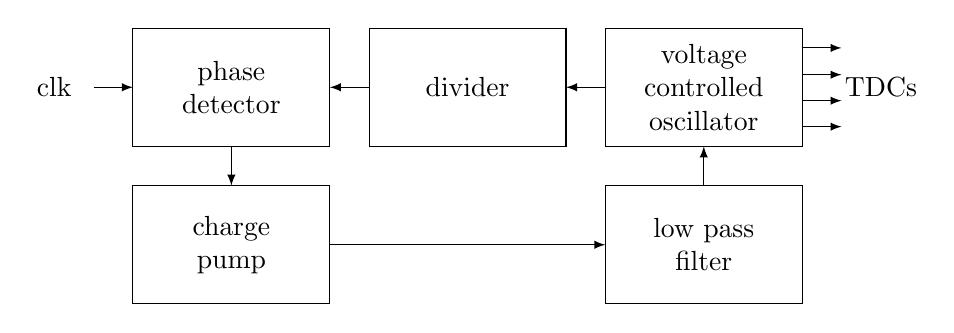
\begin{tikzpicture}

\draw  (-2,1.75) rectangle (0.5,0.25) node[pos=.5, align=center]{phase\\detector};
\draw  (1,1.75) rectangle (3.5,0.25) node[pos=.5, align=center]{divider};
\draw  (4,1.75) rectangle (6.5,0.25) node[pos=.5, align=center]{voltage\\controlled\\oscillator};
\draw  (4,-0.25) rectangle (6.5,-1.75) node[pos=.5, align=center]{low pass\\filter};
\draw  (-2,-0.25) rectangle (0.5,-1.75) node[pos=.5, align=center]{charge \\pump};

\draw [>=latex, ->] (1,1) -- (0.5,1);
\draw [>=latex, ->] (4,1) -- (3.5,1);
\draw [>=latex, ->] (0.5,-1) -- (4,-1);
\draw [>=latex, ->] (-0.75,0.25) -- (-0.75,-0.25);
\draw [>=latex, ->] (5.25,-0.25) -- (5.25,0.25);
\draw [>=latex, ->] (-2.5,1) -- (-2,1);

\draw [>=latex, ->] (6.5,1.5) -- (7,1.5);
\draw [>=latex, ->] (6.5,1.16) -- (7,1.16);
\draw [>=latex, ->] (6.5,.83) -- (7,.83);
\draw [>=latex, ->] (6.5,0.5) -- (7,0.5);


\node at (-3,1) {clk};
\node at (7.5,1) {TDCs};
\end{tikzpicture}
    \caption{schematic of phase locked loop generating signals for TDCs}
    \label{tkz:PPL}
\end{figure}

\begin{figure}[H]
    \centering


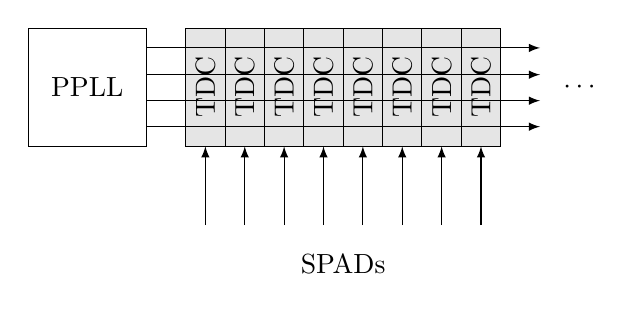
\begin{tikzpicture}

\draw  (-3.25,3) rectangle (-1.75,1.5) node[pos=.5]{PPLL};

\draw [fill=gray!20] (-1.25,3) rectangle (-0.75,1.5) node[pos=.5, rotate=90]{TDC};
\draw [fill=gray!20] (-0.75,3) rectangle (-0.25,1.5) node[pos=.5, rotate=90]{TDC};
\draw [fill=gray!20] (-0.25,3) rectangle (0.25,1.5) node[pos=.5, rotate=90]{TDC};
\draw [fill=gray!20] (0.25,3) rectangle (0.75,1.5) node[pos=.5, rotate=90]{TDC};
\draw [fill=gray!20] (0.75,3) rectangle (1.25,1.5) node[pos=.5, rotate=90]{TDC};
\draw [fill=gray!20] (1.25,3) rectangle (1.75,1.5) node[pos=.5, rotate=90]{TDC};
\draw [fill=gray!20] (1.75,3) rectangle (2.25,1.5) node[pos=.5, rotate=90]{TDC};
\draw [fill=gray!20] (2.25,3) rectangle (2.75,1.5) node[pos=.5, rotate=90]{TDC};

\draw [>=latex, ->] (-1.75,2.75) -- (3.25,2.75);
\draw [>=latex, ->] (-1.75,2.41) -- (3.25,2.41);
\draw [>=latex, ->] (-1.75,2.08) -- (3.25,2.08);
\draw [>=latex, ->] (-1.75,1.75) -- (3.25,1.75);

\draw [>=latex, ->] (-1,0.5) -- (-1,1.5);
\draw [>=latex, ->] (-0.5,0.5) -- (-0.5,1.5);
\draw [>=latex, ->] (0,0.5) -- (0,1.5);
\draw [>=latex, ->] (0.5,0.5) -- (0.5,1.5);
\draw [>=latex, ->] (1,0.5) -- (1,1.5);
\draw [>=latex, ->] (1.5,0.5) -- (1.5,1.5);
\draw [>=latex, ->] (2,0.5) -- (2,1.5);
\draw [>=latex, ->] (2.5,0.5) -- (2.5,1.5);

\node at (3.75,2.25) {$\cdots$};
\node at (0.75,0) {SPADs};
\end{tikzpicture}
    \caption{TDC line connected to PLL}
    \label{tkz:TDC_line_PLL}
\end{figure}
